\documentclass[
 reprint,
 superscriptaddress,
 amsmath,amssymb,
 aps,
]{revtex4-1}

\usepackage{graphicx}
\usepackage{dcolumn}
\usepackage{bm}
\usepackage[separate-uncertainty=true]{siunitx}
\usepackage{mhchem}
\usepackage{tikz}
\usepackage{tikzscale}

\newcommand{\rmd}{\rm{d}}
\newcommand{\diff}[2]{\frac{\rmd#1}{\rmd#2}}
\newcommand{\acf}{\rm{ACF}}
\newcommand{\angstrom}{\rm{\AA}}
\newcommand{\scinot}[2]{ {#1} \times 10^{#2} }

\begin{document}

\title{A tutorial on the model-dependent analysis of neutron and X-ray reflectometry}% Force line breaks with \\
\thanks{Modified from a document prepared for the ISIS Neutron Training Course in March 2020, which was unfortunately cancelled due to the COVID-19 pandemic}%

\author{Andrew R. McCluskey}
  \email{andrew.mccluskey@diamond.ac.uk}
  \email{a.r.mccluskey@bath.ac.uk}
  \affiliation{Diamond Light Source, Rutherford Appleton Laboratory, Harwell Science and Innovation Campus, Didcot, OX11 0DE, UK}
  \affiliation{Department of Chemistry, University of Bath, Claverton Down, Bath BA2 7AY, UK}
\author{Andrew R. J. Nelson}
  \affiliation{Bragg Institute, Australian Nuclear Science and Technology Organisation, Locked Bag 2001, Kirrawee DC, NSW 2232, Australia}
\author{Tim Snow}
  \affiliation{Diamond Light Source, Rutherford Appleton Laboratory, Harwell Science and Innovation Campus, Didcot, OX11 0DE, UK}
  \affiliation{School of Chemistry, University of Bristol, Bristol, BS8 1TS, UK}
\author{James Durant}
  \affiliation{ISIS Pulsed Neutron and Muon Source, Science and Technology Facilities Council, Rutherford Appleton Laboratory, Harwell Science and Innovation Campus, Didcot, Oxfordshire, OX11 0QX, UK}
\author{Joshaniel F. K. Cooper}
  \affiliation{ISIS Pulsed Neutron and Muon Source, Science and Technology Facilities Council, Rutherford Appleton Laboratory, Harwell Science and Innovation Campus, Didcot, Oxfordshire, OX11 0QX, UK}
\author{Juan M. Carmona Loaiza}
  \affiliation{J\"ulich Centre for Neutron Science (JCNS) at Heinz Maier-Leibnitz Zentrum (MLZ).
	Lichtenbergstraße 1, 85748 Garching, Germany.}

\collaboration{Open Reflectometry Standards Organisation}%\noaffiliation


\date{\today}% It is always \today, today,
             %  but any date may be explicitly specified

\begin{abstract}
Neutron reflectometry analysis is an inherently ill-posed problem, which is to say that there are many possible solutions which agree equally well with the measured data.
This leads to the use of model-dependent analysis to interpret the experimental data, where information that is ``known'' about the system is integrated into the analysis.
This tutorial aims to introduce the mathematics that underlies the use of model-dependent analysis in neutron reflectometry.
I hope that those that are well experienced in reflectometry find it as useful as those who are just about to experience their first reflectometry experiment.
\end{abstract}

\maketitle

% I know that it is common/precedent to start by looking at the Born approximation, but I wonder if, in paper format, it is just worth pointing out that multiple reflections invalidate Born and something iterative needs to be done? J.C.

\section{Introduction}
The mathematical concepts that underpin unpolarised reflectometry are not typically affected by whether the probing radiation is the neutron or a beam of X-rays.
Therefore, I will discuss these agnostically and only reference a given radiation source when particularly relevant.
Additionally, this work will focus only on unpolarised, nonmagnetic reflectometry analysis.
For those interested in polarised neutron reflectometry analysis, we suggest the work of Fitzsimmons, Toperverg and others \cite{fitzsimmons_applications_2005,zabel_polarized_2007,toperberg_neutron_2015}.

The collected data (once normalised) is described in terms of reflected intensity, $R(q)$, which depends on the wavevector, $q$, and is measured as,
%
\begin{equation}
    R(q) = \frac{\text{specular reflected intensity at $q$}}{\text{incident radiation intensity}},
    \label{equ:refl}
\end{equation}
%
where the denominator in Equation~\ref{equ:refl} is the total flux of X-rays or neutrons on the sample.
It is this $R(q)$ that we want to calculate from our model and then compare with our data.

The Born approximation \cite{born_quantenmechanik_1926}, which assumes a single scattering event for each incident radiation particle, allows the reflected intensity to be calculated as follows \cite{sivia_elementary_2011},
%
\begin{equation}
    R(q) \approx \frac{16\pi^2}{q^4} \bigg| \int^{+\infty}_{-\infty}{\rho'(z)\exp{(-\mathrm{i} zq) \text{d}z} \bigg|^2},
    \label{equ:kine}
\end{equation}
%
where, $\rho'(z)$ is the first derivative of the scattering length density profile.
The scattering length density profile is our model, a functional description of how the scattering length density varies with depth normal to the interface, $z$.

The approach outlined above is referred to as the kinematic approach, and it has a significant problem that can be demonstrated by considering the simple case of a bare silicon surface \cite{sivia_elementary_2011}, which can be modelled with a Heaviside function, shown in Figure~\ref{fig:kine}(a),
%
\begin{equation}
    \rho(z) =
    \begin{cases}
        0 & \text{where } z < 0,\\
        \rho_{\text{Si}} & \text{otherwise},
    \end{cases}
\end{equation}
%
%
\begin{figure}[t]
    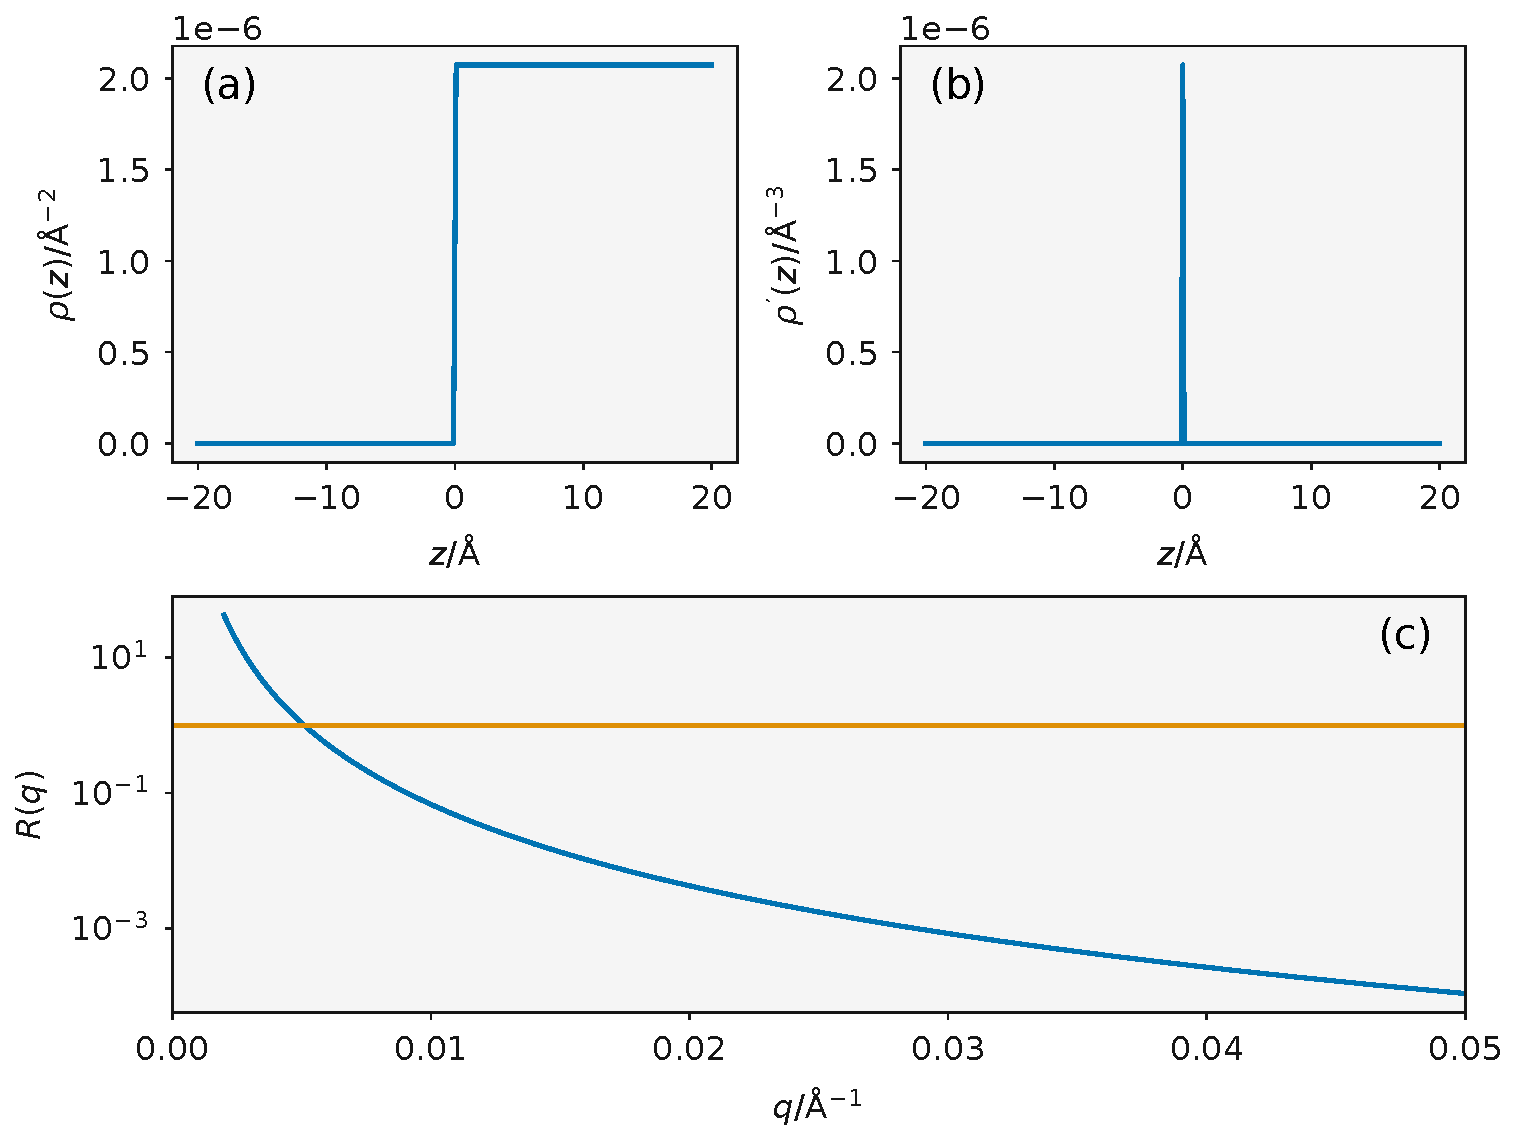
\includegraphics[width=0.49\textwidth]{kine}
    \caption{A graphical representation of each aspect of the kinematic approach; (a) the Heaviside function describing the scattering length density profile for a bare silicon substrate, (b) the $\delta$-function arising from the first derivative of the function in (a), and (c) the resulting reflectometry profile, where the orange line at $R(q)$ = 1 identifies the breakdown of between experiment and theory.}
    \label{fig:kine}
\end{figure}
%
where, $\rho_{\text{Si}} = \SI{2.074e-6}{\angstrom^{-2}}$, the nuclear scattering length density for pure silicon.
The first derivative of a Heaviside function is a scaled $\delta$-function, shown in Figure~\ref{fig:kine}(b),
%
\begin{equation}
    \rho'(z) = \rho_{\text{Si}}\delta(z).
\end{equation}
%
Then, using Equation~\ref{equ:kine}, we can calculate the reflected intensity with respect to $q$,
%
\begin{equation}
    \begin{aligned}
    R(q) & \approx \frac{16\pi^2}{q^4} \bigg| \rho_{\text{Si}}\int^{+\infty}_{-\infty}{\delta(z)\exp{(-\mathrm{i} zq) \text{d}z}} \bigg|^2 \\
     & \approx \frac{16\pi^2}{q^4} \bigg| \rho_{\text{Si}} \exp{(0)} \bigg| ^2 \\
     & \approx \frac{16\pi^2\rho_{\text{Si}}^2}{q^4}.
    \end{aligned}
    \label{equ:baresi}
\end{equation}
%
The result of Equation~\ref{equ:baresi} is shown in Figure~\ref{fig:kine}(c), where it is clear that the agreement with an experimental profile would be poor as $q \to 0$ \cite{majkrzak_exact_1998}, where the reflected intensity is greater than \num{1}.
This violates the physical condition imposed by Equation~\ref{equ:refl}, with more neutrons being reflected than were incident in the first place.
The breakdown of this kinematic approach is due to the assumption of the Born approximation that each incident radiation particle is only scattered once.
The reflectometry geometry, where a large path length arises from the shallow incidence angle means that multiple scattering events are likely, rendering the kinematic approach invalid.

\section{Recursive methods}
The breakdown of the kinematic approach leads to the application of the Abel\`{e}s \cite{abeles_sur_1948} or Parratt \cite{parratt_surface_1954}, recursive model for the reflection of light at a given number of stratified interfaces, also referred to as the dynamical approach.
This is an alternative method for calculating the reflected intensity from a model, however, now the model is a series of layers of different scattering length density.
The probing radiation can be either reflected or refracted at the interface between each of the layers.
%
\begin{figure}[t]
    \includegraphics[width=\linewidth]{dynamic}
    \caption{A schematic diagram showing the reflected ($r$) and transmitted ($t$) waves when an incident ($i$) wave enters an interface of thickness $d$.}
    \label{fig:refr}
\end{figure}
%
Figure~\ref{fig:refr} shows the refraction and reflections from a simple two layer system, where layer \num{0} is a vacuum above the sample.
It is clear, by analogy to Bragg's law, how the two waves, labelled $r$, could interfere constructively or destructively depending on the thickness of layer \num{1}, $d$.

The generalisation of this approach to any number of layers is possible and enables the reflected intensity to be calculated at each value of $q$ that was measured.
The incident neutrons will be refracted by each of the layers, giving wavevectors for each layer, $k_n$,
%
\begin{equation}
    k_n = \sqrt{k_0+4\pi(\rho_n - \rho_0)},
\end{equation}
%
where, $k_0 = 0.5q$.
The Fresnel equation coefficient between layers $n$ and $n+1$, $r_{n, n+1}$, can then be found along with the phase factor, $\beta_n$, for the layer $n$,
%
\begin{equation}
    r_{n, n+1} = \frac{k_n - k_{n+1}}{k_n + k_{n+1}},
    \label{equ:fres}
\end{equation}
%
%
\begin{equation}
    \beta_n = k_nd_n.
\end{equation}
%
From the Fresnel equation coefficient and phase factor, a characteristic matrix for each layer, $M_n$, can be constructed,
%
\begin{equation}
    M_n =
    \begin{bmatrix}
        \exp{\beta_n} & r_{n,n+1}\exp{-\beta_n} \\
        r_{n,n+1}\exp{\beta_n} & \exp{-\beta_n}
    \end{bmatrix},
\end{equation}
%
and the resultant matrix for a given $q$-vector, $B(q)$ is found from the product sum of the matrices from each layer,
%
\begin{equation}
    B(q) = \prod_{n=0}^{n_{\text{max}}}{M_n}.
\end{equation}
%
The characteristic matrix for each layer describes the reflected and refracted radiation intensity, so the product sum is able to describe the total reflected intensity.
In particular, this is given by the following elements of the resultant matrix,
%
\begin{equation}
    R(q) = \frac{B_{1,2}(q)}{B_{1,1}(q)}.
\end{equation}
%

This algorithm models the layers as perfectly flat layers, which may not be strictly true.
This has resulted in the use of correction terms to be added to Equation~\ref{equ:fres} to account for this roughness.
The most common of these is N\'{e}vot and Croce Gaussian broadening \cite{nevot_caracterisation_1980}, in which the Fresnel equation coefficient is evaluated as,
%
\begin{equation}
    r_{n, n+1} = \frac{k_n - k_{n+1}}{k_n + k_{n+1}} \exp{(-2k_nk_{n+1}\sigma^2_{n,n+1})},
\end{equation}
%
where, $\sigma_{n, n+1}$ is the interfacial roughness between the layers $n$ and $n+1$.
Applying this dynamical approach to a perfectly flat silicon surface is shown in Figure~\ref{fig:dyna}.
There is a clear difference between the kinematic and dynamical approaches as $q \to 0$, with the dynamical approach adhering to the physical constraint that causes the breakdown of the kinematic approach.
%
\begin{figure}[t]
    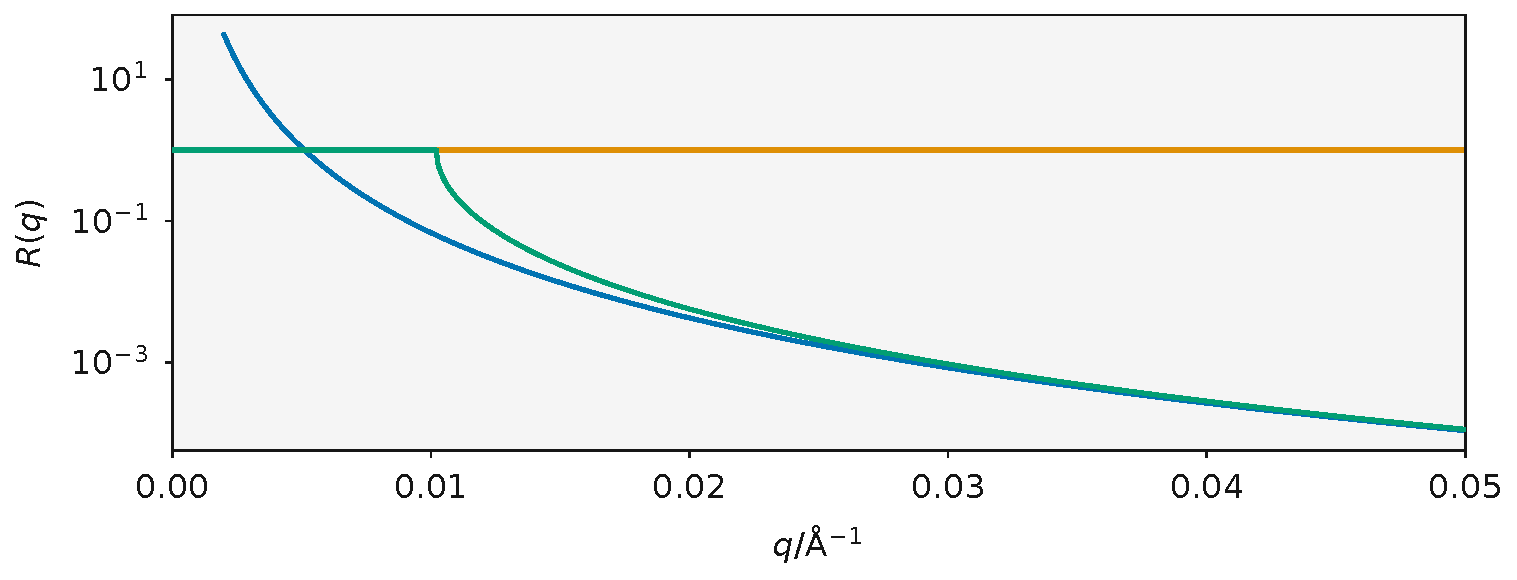
\includegraphics[width=0.49\textwidth]{dyna}
    \caption{A comparison of the kinematic (blue) and dynamical (green) approaches to determine the reflected intensity from the material with the scattering length density profile given in Figure~\ref{fig:kine}(a).}
    \label{fig:dyna}
\end{figure}
%

Figure~\ref{fig:rough} shows the effect that increasing roughness can have on the scattering length density of some system, in this case \ce{D2O} on a silicon substrate.
Notice that as the roughness gets to values similar to half the layer thickness, artifacts appear in the scattering length density profile.
Below, where the roughness is too large, the scattering length density is less then the substrate scattering length density.
This is unphysical, and indicates at an important factor that we should try and account for by not allowing large roughnesses with respect to the layer thickness, a common rule of thumb is to use less than one quarter of the layer thickness.
%
\begin{figure}[t]
    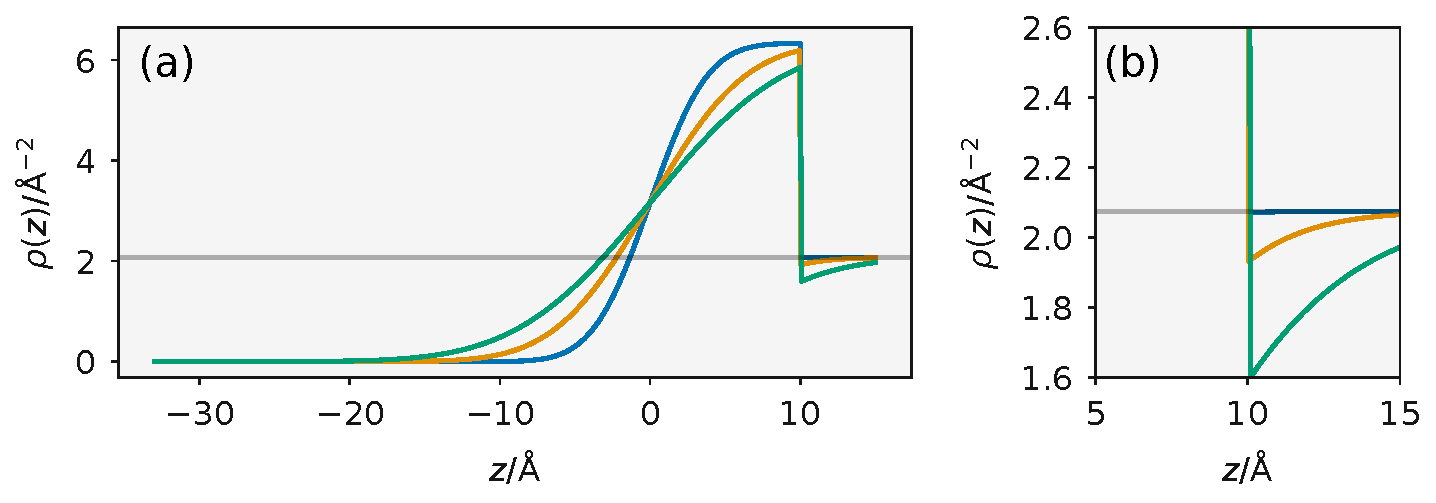
\includegraphics[width=0.49\textwidth]{roughness}
    \caption{The effect of a roughness greater than a given layer's thickness on the scattering length density profile. The layer thickness is \SI{10}{\angstrom}. The scattering length densities are those of \ce{D2O} on a atomically flat silicon. The roughness of the water layer is varied from \SI{3}{\angstrom} (blue), through \SI{5}{\angstrom} (orange), to \SI{7}{\angstrom} (green). The full scattering length density profile is given in (a), while (b) represents a zoomed in representation.}
    \label{fig:rough}
\end{figure}
%

\section{Instrumental resolution}
In the analysis process, a resolution function associated with the instrumentation the reflectometry measurement was performed on it typically introduced to the model.
This ensures greater accuracy in the modelled reflectometry to the experiment.
These resolution functions are non-trival to define, however, the majority of reflectometry instruments will be able to offer information about the appropriate function to use.

Here, we will briefly discuss the introduction of a simple Gaussian resolution function with a constant $\frac{\text{d}q}{q}$.
The Gaussian function is centred on a given wavevector, $q$, and has a width of at half maximum of $\text{d}q$.
For each $q$-value in the unsmeared data, a Gaussian function is produced which is convolved with the unsmeared to produce data that includes some description of the instrumental resolution.
Typically, this convolvutional smearing is included in the reading of the experimental data.
However, the resolution function used by a given software package may not be an accurate description of that from the instrument, therefore, we recommend discussing this with the members of instrument staff.
More information about the resolution function can be found in the work of van Well and Fredrikze \cite{vanwell_resolution_2005} and Nelson and Dewhurst \cite{nelson_towards_2013,nelson_towards_2014}

\section{Ill posedness - the phase problem}

Figure \ref{fig:phase_problem_sld} shows two hypothetical samples of the same total thickness, consisting of one and two layers, deposited on a substrate with $\rho_s = \SI{2.07e-6}{\angstrom^{-2}}$.
Even though the scattering length density depth profiles are distinctly different, the resultant reflectivity curves are virtually identical, with only a slight discrepancy at the first minimum.
This ambiguity, known as \emph{the phase problem}, is an example of the information lost in diffraction experiments due to the inability of measuring the phase of the scattered wave (note that equation \ref{equ:kine} involves a modulus-squared).
\begin{figure}
    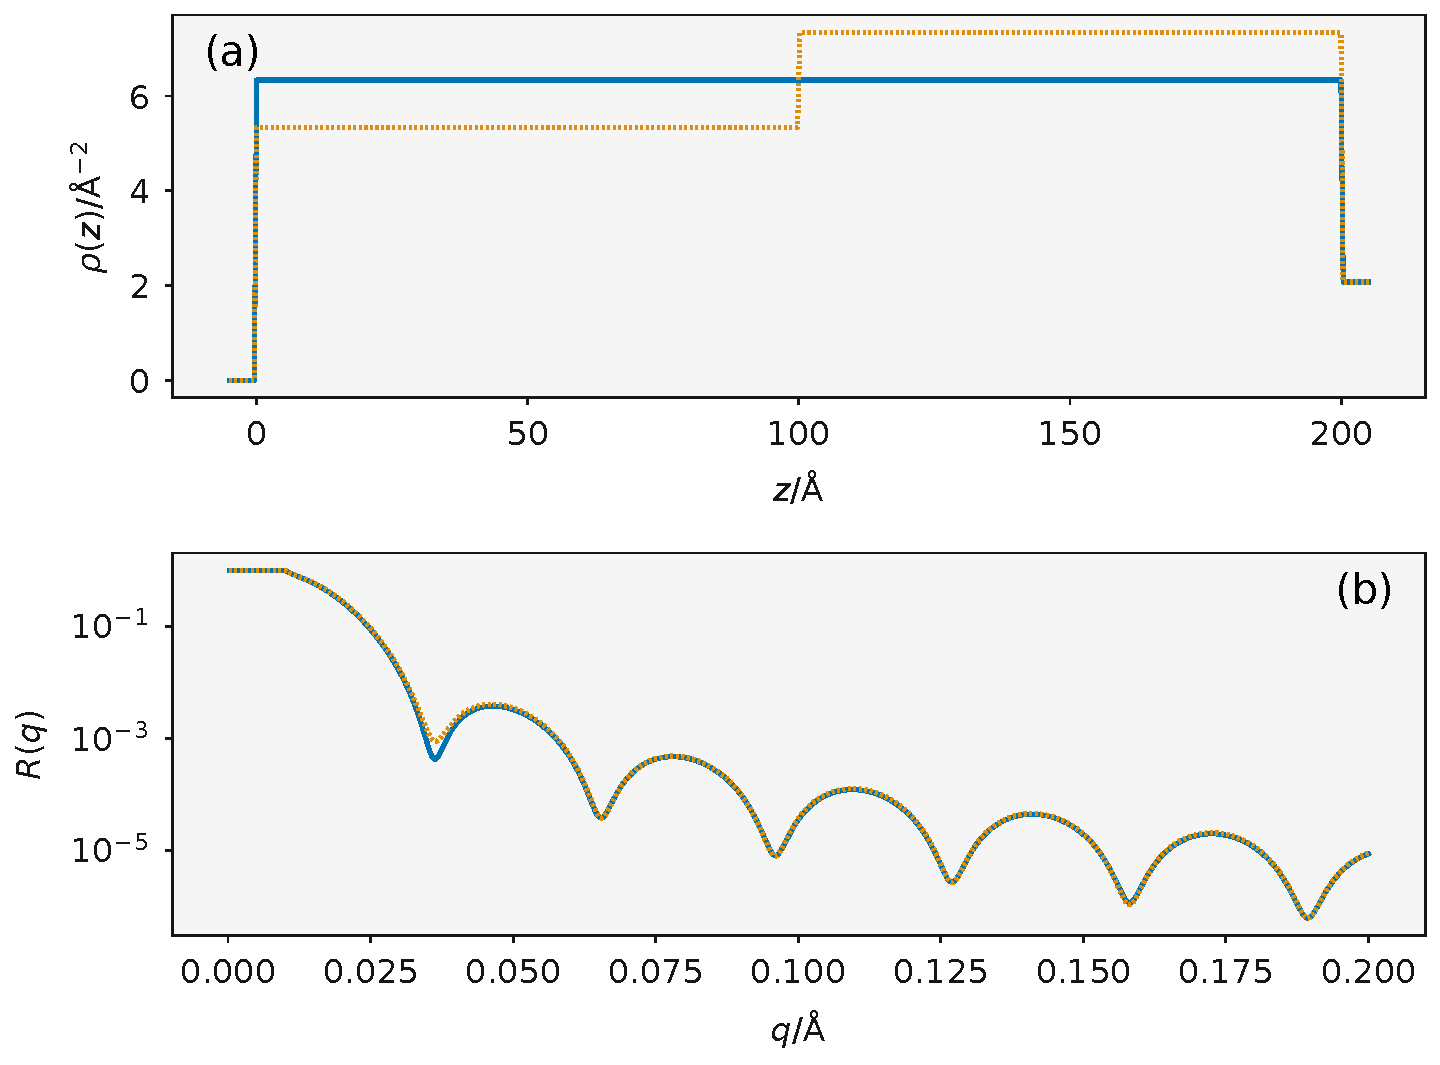
\includegraphics[width=0.49\textwidth]{phase_problem_SLD.pdf}
    \caption{The phase problem, (a) two different samples deposited on the same substrate with a scattering length density of $\rho_s$, (b) are indistinguishable from one another by looking only at their reflectivity curve $R(q)$.}
    \label{fig:phase_problem_sld}
\end{figure}

A heuristic explanation for the phase problem can be built in terms of the auto-correlation function of $\rmd\rho/\rmd z$, which gives a real-space representation of the information contained in the reflectivity pattern,
%
\begin{equation}
    \begin{aligned}
        \acf_{\rho'}(z) & = \int_{-\infty}^{\infty} \rho'(z)^* \, \rho'(z + \xi) \, \rmd \xi \\
                        & = \int_{-\infty}^{\infty} \left| \widehat{\rho'}(q)  \right|^{2} \rm{e}^{iqz} \rmd q,
    \end{aligned}
    \label{equ:acf}
\end{equation}
%
where the hat notation indicates a Fourier transform, the star notation a complex conjugate, and the prime notation a derivative.
\begin{figure}
    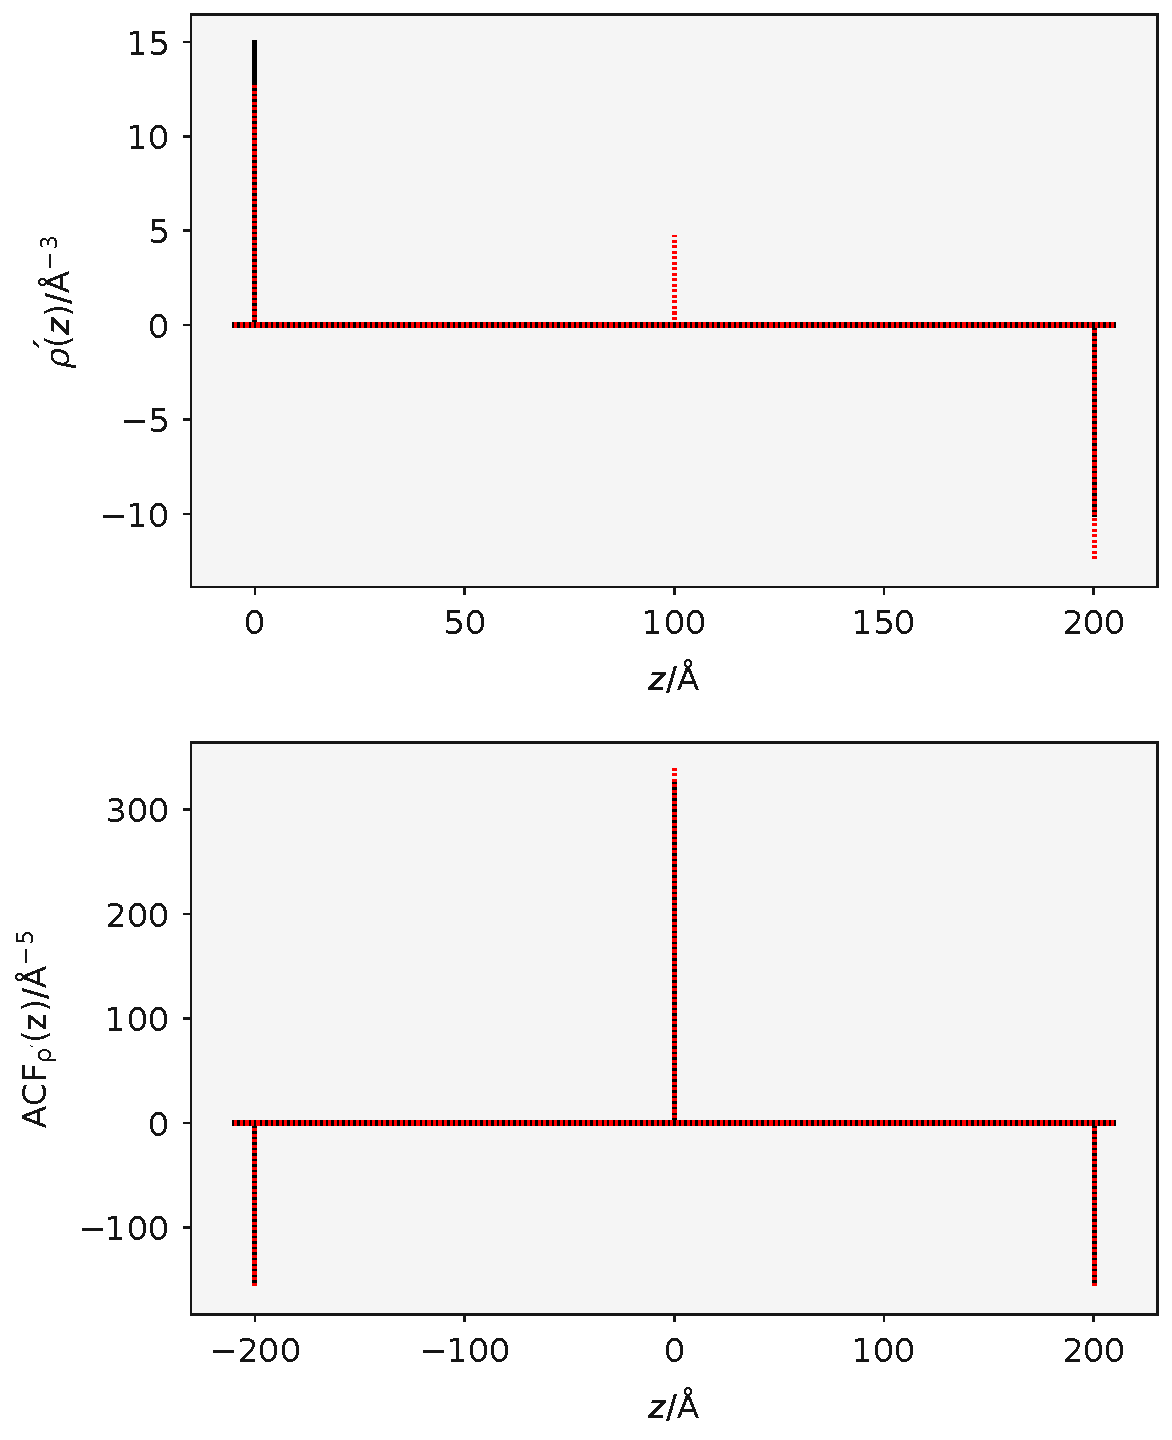
\includegraphics[width=0.49\textwidth]{phase_problem_ACF.pdf}
    \caption{The phase problem explanation: (a) the derivatives of the two hypothetical scattering length density profiles from Figure~\ref{fig:phase_problem_sld} are scaled $\delta$ functions peaking at the interfaces between scattering length density layers, (b) the autocorrelation functions, $\acf_{\rho'}(z)$ are almost identical between the samples, peaking at exactly the same locations.}
    \label{fig:phase_problem_acf}
\end{figure}

As $\rho'(z)$ is purely real and in both examples is only composed of $\delta$ functions, the ACF can be obtained by direct inspection (See Figure~\ref{fig:phase_problem_acf} and Equation~\ref{equ:acf}):
\begin{itemize}
    \item At zero lag, there is always full correlation, thus the ACF will have a large positive peak at the origin for both samples.
    \item For both samples, the interference between the front and back interfaces, at $z = 0$ and $z = \SI{200}{\angstrom}$ respectively, translates into a pair of $\delta$ peaks with opposite signs in $\rho'$. Thus, at a $\xi = \pm \SI{200}{\angstrom}$ lag, the ACF must peak with negative amplitude.
    \item For the two-layer sample, an extra pair of peaks in the ACF could be expected at lags of $\xi = \pm \SI{100}{\angstrom}$; however, since there is a complete cancellation between the positive and the negative contributions of the $\delta$ functions at $z = 0$ and $z = \SI{200}{\angstrom}$, the expected extra pair of peaks is absent.
\end{itemize}
As the scattering length density profiles of both samples translate into the same ACF, it is now not surprising the similarity between their reflectivity curves.

A deeper discussion on the phase problem and some techniques that have been developed to tackle it are described in the work by Majkrzak \emph{et al.} \cite{majkrzak_phase_2003}, who give an overview of several phase-sensitive experimental methods and claim that any ambiguity in a scattering length density profile obtained by these is a consequence only of the limited $q$ range over which reflectivities can be measured.
In a similar fashion, Koutsioubas \cite{koutsioubas_model_2019} proposes a model-independent method that, when applied to multiple solvent contrast data, should lead to reliable reconstructions of the interfacial structure without the need for any a priori assumptions.

However, even when the phase problem can be theoretically alleviated, reflectivity curves from different scattering length density profiles may still be close enough to one another to be indistinguishable by finite-resolution experiments, effectively keeping the analysis of reflectometry profiles in the realm of ill-posed non-invertible problems.
As such, reflectometry data analysis demands for advanced trial-and-error fitting techniques, the daily bread of experimenters to which the following section is devoted.

\section{Global optimisation}
The recursive method described above gives an accurate method to obtain a model reflected intensity.
However, this is just the first step in the analysis of a neutron reflectometry dataset.
Now we are interested in optimising our model such that the reflected intensity from it matches our experimental data as best as possible.
This is the problem of parameter optimisation, which is a broad area of mathematics and computer science that we will not dwell on here.
However, we will introduce the basics of optimisation and discuss the most common global optimisation method used in reflectometry.

When we measure a reflectometry profile, we measure the reflected intensity, and some uncertainty in that measurement, at discrete points in the wavevector, $R(q) \pm \delta R(q)$.
Using the recursive method discussed above, we can calculate a model reflected intensity at these same $q$ values, $R_m(q)$.
We then aim to reduce the difference between the measured and modelled reflected intensity through the optimisation (maximisation) of the likelihood, $L$,
%
\begin{equation}
    \begin{aligned}
        L = \exp\bigg\{ & - \frac{1}{2} \sum_{q=q_{\text{min}}}^{q_{\text{max}}} \bigg[\frac{R(q) - R_m(q)}{\delta R(q)}\bigg]^2 \\
         & + \ln[2\pi \delta R(q)]\bigg\}.
    \end{aligned}
\end{equation}
%
This parameter described the probability that the model $m$ accurately describes the observed reflectometry data.
The aim in reflectometry modelling is to obtain a model reflectometry that has the maximum likelihood possible for the given experimental data.
Figure~\ref{fig:likelihood} shows the maximum likelihood model for some experimental data, in addition to another model which does not agree well with the data and therefore has a lower likelihood as a result.
%
\begin{figure}[t]
    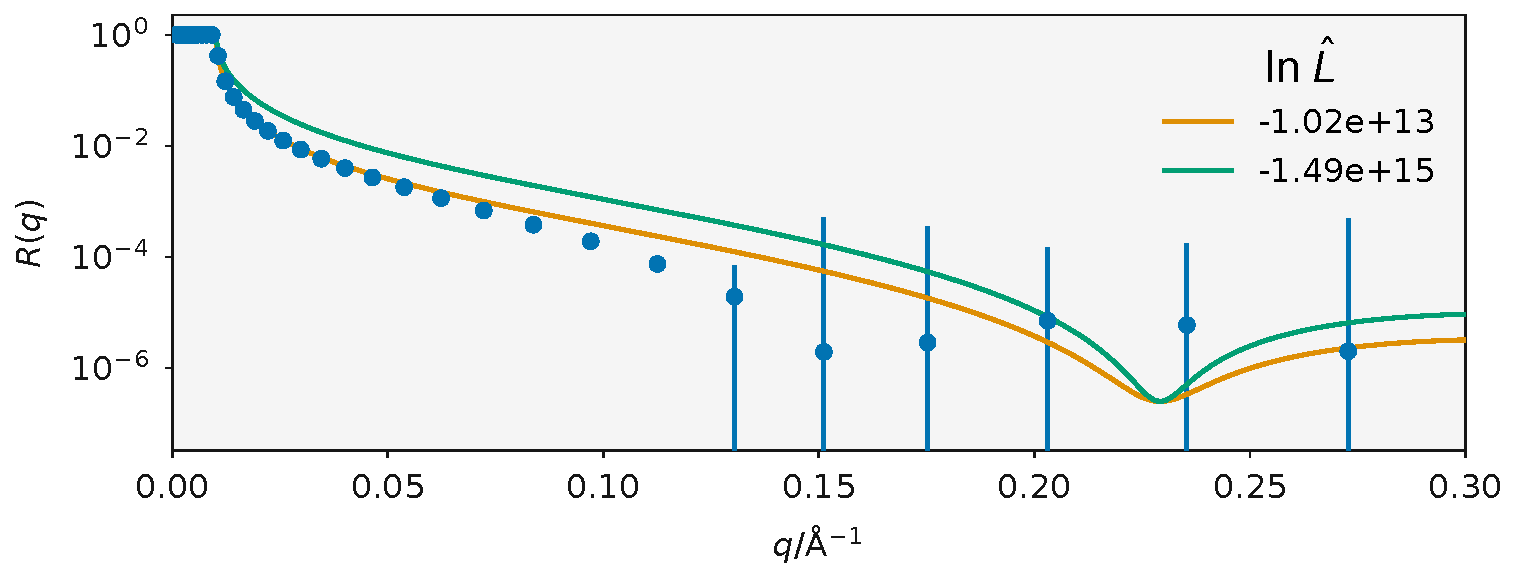
\includegraphics[width=0.49\textwidth]{likelihood}
    \caption{The maximum likelihood fit, the blue data points indicate some experimental data, while the yellow line shows the maximum likelihood model fit to this dataset and the green line show another model (which doesn't maximise the likelihood).}
    \label{fig:likelihood}
\end{figure}
%

The global optimisation of a reflectometry model is a particularly difficult problem, this is due to the ill-posed nature of this data, this is where there are many reasonable solutions to a particular reflectometry profile.
However, a particular global optimisation method has shown substantial utility in the fitting of reflectometry data \cite{varderlee_comparison_2007}: differential evolution \cite{wormington_characterization_1999}.
This has lead to the inclusion of this method in many common reflectometry analysis packages \cite{bjorck_fitting_2011}.

Differential evolution is an iterative, genetic algorithm, designed to mimic the evolution processes observed in biology \cite{holland_adaptation_1992}.
The method consists of two vectors, the parent population $\mathbf{p}$, and the offspring population, $\mathbf{o}$.
These vectors are of shape $(i \times j)$, where $i$ is the number of parameters in the model and $j$ is the number of candidate solutions being considered.
The offspring population is generated as a result of some trail method, here we will discuss only a simple classical trail method.

A classical trail method consists of two stages, mutation and recombination.
The mutation stage involves the creation of a mutant population, $\mathbf{m}$.
The magnitude of the mutation is dependent on the first of our hyperparameters, the mutation constant, $k_m$,
%
\begin{equation}
    \mathbf{m}_{i,j} = b_i + k_m (\mathbf{p}_{i, R1} - \mathbf{p}_{i, R2}),
\end{equation}
%
where $b$ is the candidate solution with the greatest likelihood, and $\mathbf{p}_{i, R1}$ and $\mathbf{p}_{i, R2}$ are randomly chosen members of the parent population.
The mutation constant hyperparameter controls the size of the search space, with a large $k_m$ corresponding to a wider search.

The recombination step creates the offspring population vector by taking a sample from either the parent or mutant population with some frequency, which depends on our second hyperparameter, the recombination constant, $k_r$,
%
\begin{equation}
    \mathbf{o}_{i, j} =
    \begin{cases}
        \mathbf{m}_{i, j} & \text{where } X < k_r,\\
        \mathbf{p}_{i, j} & \text{otherwise},
    \end{cases}
\end{equation}
%
where, $X$ is a random number selected from a uniform distribution between 0 and 1.
The recombination constant hyperparameter controls the mutation frequency in the offspring population.

The final stage is to compare the offspring and parent population vectors, in the selection stage, to create the parent population for the next iteration.
Here, the likelihood is used to compare between subunits from the offspring or parent populations,
%
\begin{equation}
    \mathbf{p}_{*, j} \leftarrow
    \begin{cases}
        \mathbf{o}_{*, j} & \text{where } L_{\mathbf{o}_{*, j}} > L_{\mathbf{p}_{*, j}},\\
        \mathbf{p}_{*, j} & \text{otherwise},
    \end{cases}
\end{equation}
%
where, the $*, j$ subscript notation indicates all objects from the population, $j$.
Following the use of the differential evolution algorithm, typically a more common (gradient-based) approach is used to ensure that the likelihood has been maximised within the space identified by the differential evolution.

The differential evolution algorithm can be seen in action applied to the negative two-dimensional Ackley function \cite{ackley_connectionist_1987}, in Figure~\ref{fig:ackley}.
The Ackley function is a common function used in the assessment of global optimisation functions. This is due to there being a large number of local minima and only a single global minimum to this function. Here, we want to maximise the value, so the negative Ackley function is used.
This function can maximise the value of the negative Ackley function.
While this does not offer a clear example of this algorithm's application to reflectometry analysis, the popularity of this method in the fitting of reflectometry profiles cannot be denied \cite{bjorck_fitting_2011,nelson_refnx_2019}.
%
\begin{figure}[t]
    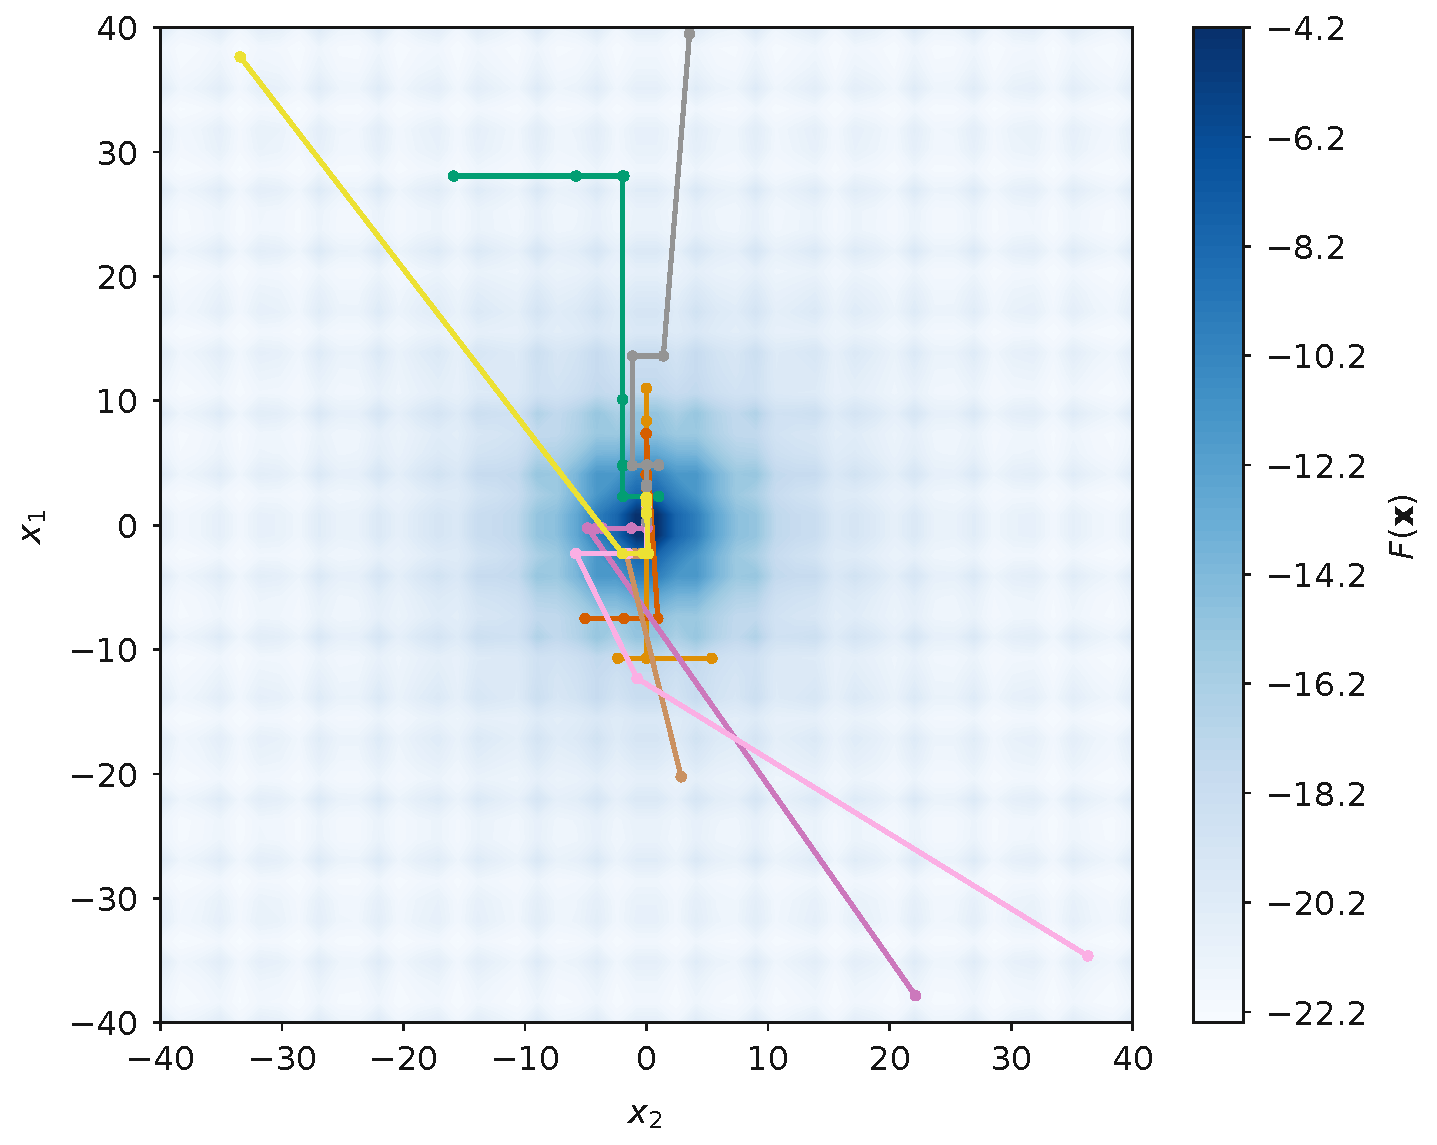
\includegraphics[width=0.49\textwidth]{ackley}
    \caption{An example of a differential evolution algorithm applied to the negative of an Ackley function. In this implementation $k_m=0.5$ and $k_r=0.5$. Each line represents a different candidate solution. The optimisation was stopped after 100 iterations had run.}
    \label{fig:ackley}
\end{figure}
%

The analysis of a reflectometry model can take advantage of contrast variation, the exact methods of which are covered in other articles \cite{schurtenberger_contrast_2002}.
However, we note here that, the phrase ``global optimisation'' is often used to describe the analysis of multiple contrasts of the same structure.
This is where a single structural model is used for the analysis of multiple measurements, but the scattering length densities are varied based on the particular contrasts under investigation.
This method has been used to recover the phase information in neutron reflectometry analysis \cite{majkrzak_exact_1995,majkrzak_first_2000,majkrzak_phase_2003,koutsioubas_model_2019}.
However, it is also a tool in model-dependent analysis, as it reduces the number of local minimia in the parameter space.
Typically, a global (here meaning multiple contrasts) optimisation criteria is used. For example, the average or summed likelihood across all of the different measurements and model reflectometries.

\section{Uncertainty quantification}
Reflectometry measurements offer an average description of the out of place structure of a material.
This means that it is pragmatic to describe the uncertainties in the values of our model parameters in some fashion.
In this section, we will introduce two potential methods to determine the uncertainty on a set of model parameters.

The first is computationally straightforward and is substantially more common.
This is where the parameter uncertainties are found from the Hessian matrix of the optimisation space, where the uncertainties are the square-root of the matrix diagonal.
The previous sentence introduced a lot a terminology that may not be familiar, however we shall work through it slowly.
The above optimisation method, differential evolution, is what is referred to as a stochastic method, where steps taken arise from a randomly determined process.
However, another common type of optimisation methods are known as gradient methods, where the gradient of the optimisation space at a given point is calculated and this is used to determine the next position.
Consider maximising the likelihood for a reflectometry model fit, you would like to make steps that increase the likelihood to reach the maximum, so calculating the gradient will be able to tell you in which direction to travel.

The Hessian matrix, $H$ describes the curvature of optimisation criteria, the likelihood, with respect to each of the model parameters, and it is frequently used in the gradient-based optimisation methods.
This means it is an $i\times i$ matrix, where $i$ is again the number of model parameters, $\theta$. For a two parameter model, this would look like,
%
\begin{equation}
    H =
    \left[\begin{matrix}
        \dfrac{\partial^2 L}{\partial \theta_{1}^2} & \dfrac{\partial^2 L}{\partial \theta_1 \theta_2} \\[6pt]
        \dfrac{\partial^2 L}{\partial \theta_2 \theta_1} & \dfrac{\partial^2 L}{\partial \theta_{2}^2}
    \end{matrix}\right].
\end{equation}
%
If the parameter distribution is Gaussian in shape then the second derivative at the Gaussian maximum will give the variance of that distribution.
Therefore, when these gradient approaches are used, the Hessian matrix is calculated and the diagonal of that matrix gives the uncertainty in each of the parameters.
The off-diagonal elements contain information about the covariance between different parameters, however this is rarely leveraged and the covariances are taken to be negligible.
Additionally, we note that often the Hessian is not calculated in an optimisation so the Jacobian matrix (the first derivative analogue of the Hessian) is used to estimate Hessian matrix.

The determination of parameter uncertainties from the Hessian matrix is dependent on two major assumptions about the parameter space:
\begin{enumerate}
    \item {the parameters are normally distributed with a single maximum,}
    \item {the covariance between the parameters is negligible.}
\end{enumerate}
However, this may not always be the case \cite{mccluskey_bayesian_2019}. Therefore, is it necessary to use methods to completely describe the parameter probability distribution.
One such method for this is Markov-chain Monte Carlo (MCMC), which samples the posterior probability distribution for each of our parameters to obtain an analytical description \cite{sivia_data_2006}.
Typically, MCMC is used on already optimised solutions to a particular problem. In reflectometry analysis it is usually applied after the differential evolution has optimised the structure.
In addition to being able to quantify the inverse uncertainties (the name given to the uncertainties in the model parameters) MCMC also offers a more complete understanding of the correlations between different parameters \cite{gilks_markov_1995}, which is particularly important in the ill-posed reflectometry analysis.

Once an optimised set of model parameters, $\theta$, are obtained which maximise the likelihood, $L$, some random perturbation is applied,
%
\begin{equation}
    \Theta = \theta + aR,
\end{equation}
%
where $R$ is some normally distributed number centered on \num{0} with a standard distribution of \num{1} and $a$ is the step size.
A new $L$ is found for $\Theta$ and the probability that this transition is will occur is found,
%
\begin{equation}
    p = \exp{\bigg[\frac{L(\Theta) - L(\theta)}{2}\bigg]}.
\end{equation}
%
This probability is then compared with a uniformly distributed random number from \num{0} to \num{1}, $n$,
%
\begin{equation}
    \theta \leftarrow
    \begin{cases}
        \Theta & \text{where } n < p,\\
        \theta & \text{otherwise}.
    \end{cases}
\end{equation}
%
This process is repeated until some desired number of samples has been obtained.
It should be noted that it is important to allow the Markov chains to have some ``burn-in'' period, which is not included in the final samples.
This allows the MCMC algorithm to settle into the search-space.

Figure~\ref{fig:mcmc} shows the result of a MCMC sampling for a pair of overlapping Gaussian functions, performed using the \texttt{emcee} Python package \cite{foremanmackey_emcee_2012}.
The posterior probability distributions that are available to each of the four parameters are shown along with the data, the optimised fit and a subset of models within the posterior distributions.
All of the samples from the posterior distributions fit within the uncertainty error bars on the data.
This shows the ability for MCMC to sample the range of the distribution that is allowed by the experimental uncertainty.
%
\begin{figure}[t]
    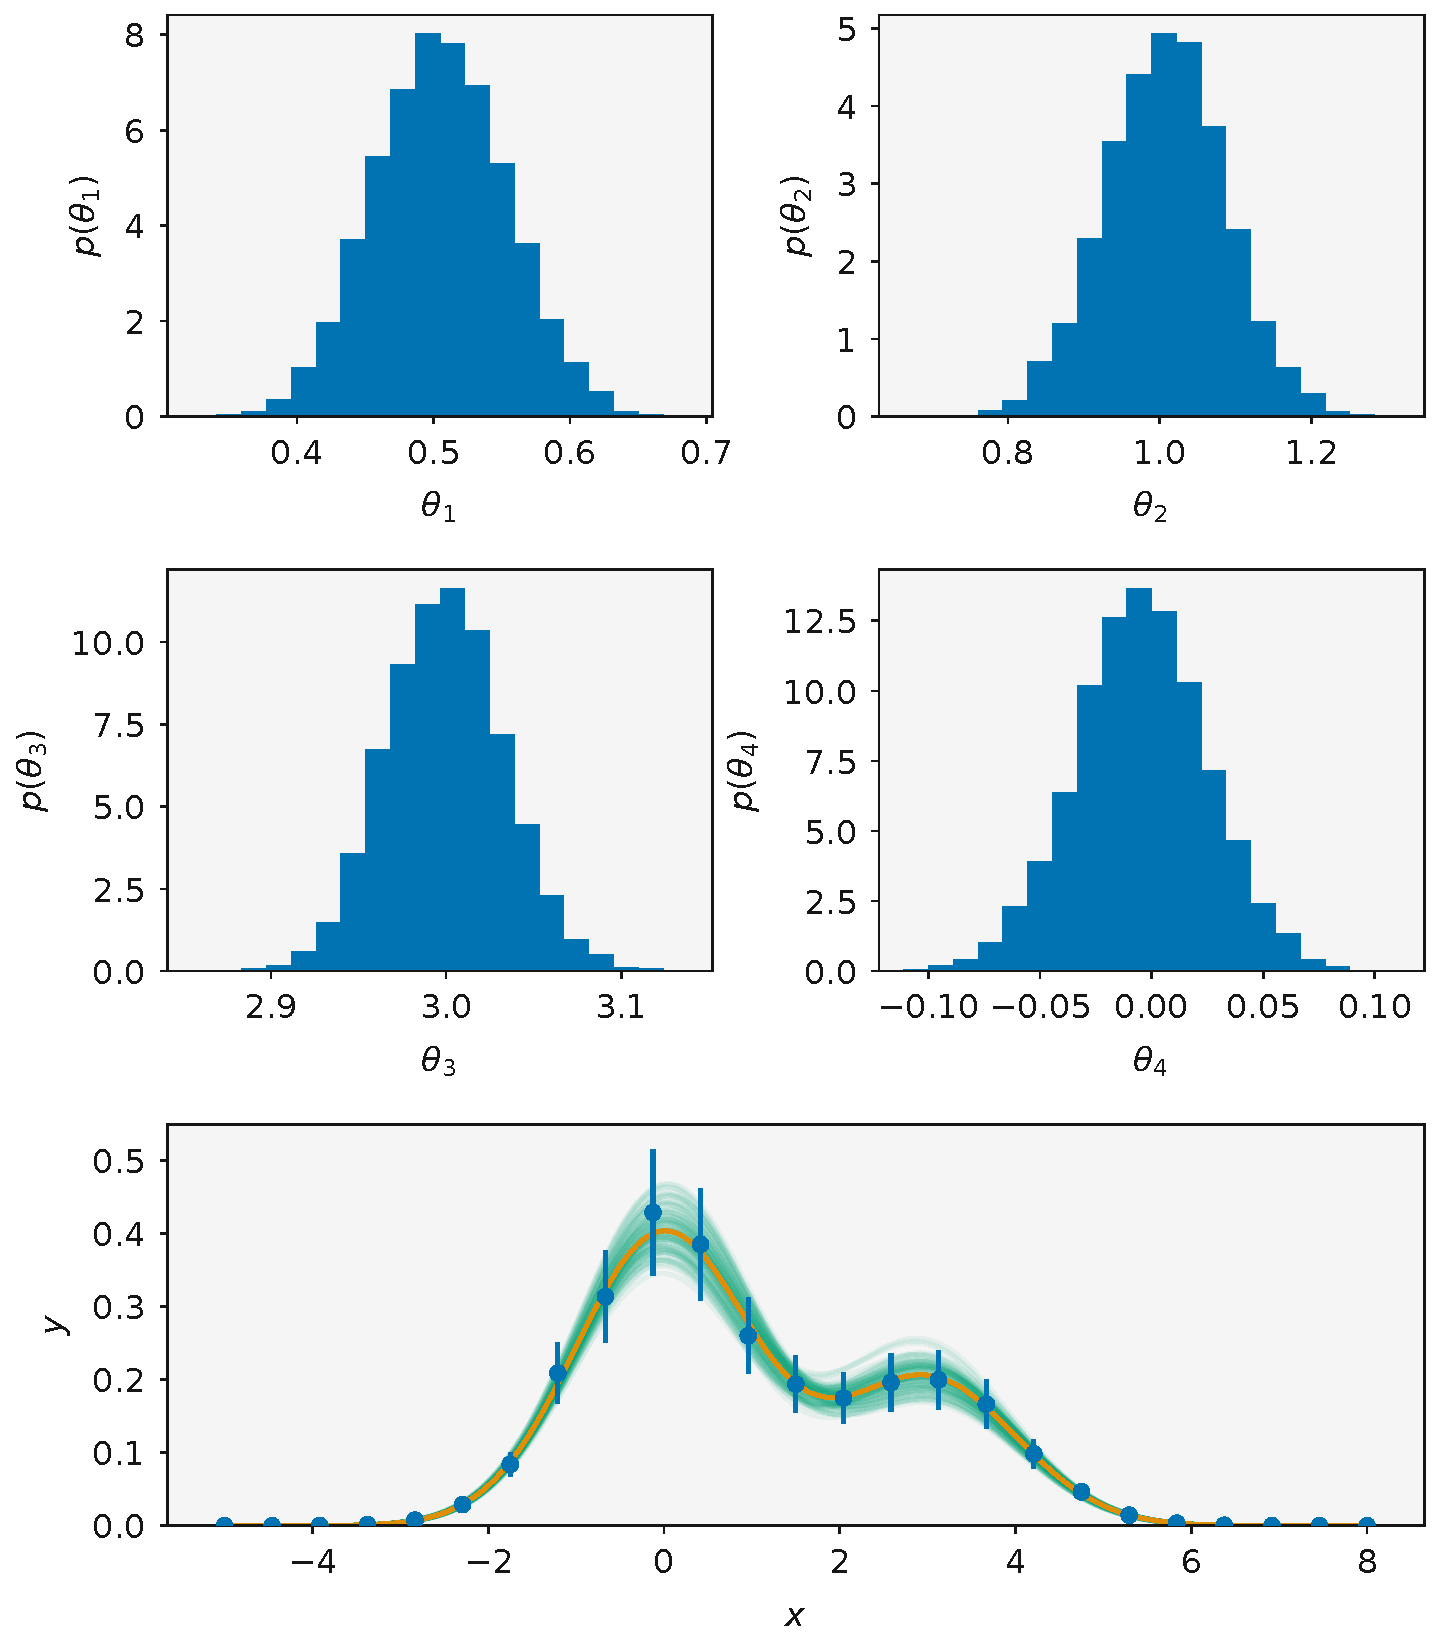
\includegraphics[width=0.49\textwidth]{mcmc}
    \caption{An example of the result of MCMC uncertainty sampling on data synthesized from two overlapping Gaussian functions. $\theta_1$ and $\theta_2$ are the integrals of the Gaussian functions while $\theta_3$ and $\theta_4$ are the positions. The data is shown with blue circles, the optimised model with an orange line, and samples from the posterior distributions with green lines.}
    \label{fig:mcmc}
\end{figure}
%

We note here that MCMC may also be used to facilitate the use of Bayesian inference in the analysis of reflectometry data, where other prior knowledge about the experimental system is able to influence the result of the analysis.
In this tutorial, we won't say any more on this subject, but if you are interested, this is discussed in the work of Nelson and Prescott \cite{nelson_refnx_2019} and McCluskey and co-workers \cite{mccluskey_general_2020}.

\section{Conclusions}
The aim of this document was to give an introduction to some of the mathematical concepts that underpin modern reflectometry model-dependent analysis.
We have looked at how reflectometry is calculated from a layer model description of the scattering length density profile, and why the kinematic approach fails.
Then we have discussed the importance of the differential evolution algorithm in reflectometry analysis and detailed the operation of this algorithm.
Finally, Markov-chain Monte Carlo was introduced in the context of uncertainty quantification for model-dependent analysis, with particular importance for reflectivity discussed.
While not exhaustive, I hope that this document will give you the confidence in understanding to look in more detail into how the analysis of reflectometry measurements are performed.

\section*{Author Contributions}
ARM wrote the first draft of this text, and ARJN and TS offered input on additional content to cover and clarifications to include.


proposed, implemented, and applied the Bayesian model comparison framework, with input from T.A., J.F.K.C. and T.S.; J.F.K.C. and T.S. sourced funding; A.R.M. wrote the manuscript, with input from all authors.


\section*{Acknowledgements}
ARM is supported by the Ada Lovelace Centre -- a joint initiative between the Science and Technology Facilities Council (as part of UK Research and Innovation), Diamond Light Source, and the UK Atomic Energy Authority.
The authors would like to thank Luke Clifton of ISIS Neutron and Muon Source for insightful input on the manuscript.


\bibliography{handout}
\bibliographystyle{unsrtnat}

\end{document}
